
\section{ByteNet}

\subsection{Validating Implementation}

Before using the model on the Europarl v7 dataset for solving the WMT Translation Task problem, the model is validated using some simpler datasets.

\subsubsection{Learning Synthetic Digits Problem}

The Synthetic Digits dataset is used for validating the generalization properties of the ByteNet implementation. The internal dimensionality is set to 20, this is 20 units in the encoder and 40 units in the decoder, the latter is because the encoding is concatenated with the target embedding. The ByteNet model is optimized using the MaxProp optimizer with a learning rate of 0.01.

Because the BLEU score is not meaningful for the Synthetic Digits problem, where no words exists in the target, the misclassification rate is calculated instead.

\begin{figure}[H]
    \centering
    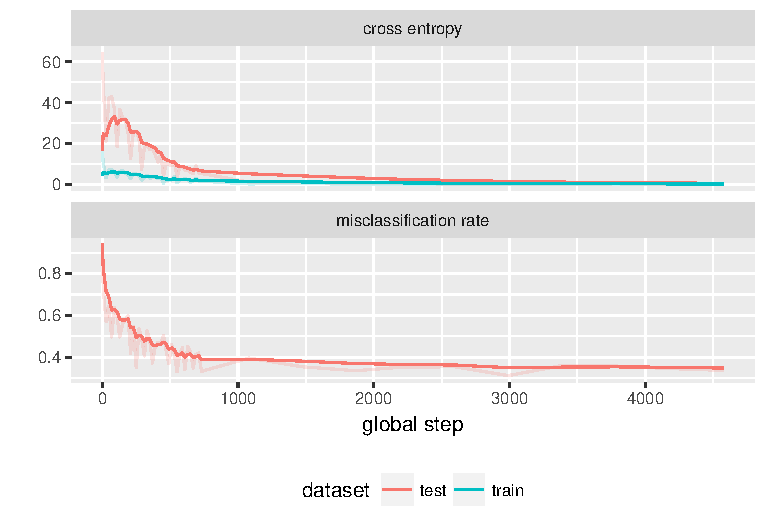
\includegraphics[scale=1]{bytenet/validation-synthetic-digits.pdf}
    \caption{Shows misclassification rate and the cross entropy loss. The training size is set to 128 observations, likewise for the test dataset. For comparison a the attention model has misclassification rate at 0.51.}
\end{figure}

\begin{table}[h]
\centering
\begin{tabular}{r|p{3.3cm} p{3.3cm} p{3.3cm}}
	obs. & source & target & predict\\ \hline
  0 & one zero four & 104 & 104 \\
  1 & one five six & 156 & 15 \\
  2 & five five nine & 559 & 559 \\
  3 & one six & 16 & 10 \\
  4 & two three four & 234 & 212 \\
  5 & five three & 53 & 53
\end{tabular}
\caption{Source, target and prediction on the test dataset.}
\end{table}

\clearpage
\subsubsection{Memorizing WMT NewsTest}

Sometimes a model works well when it has few weights, but breaks for higher dimensionality because of vanishing or exploding gradient issues. A good test is to see if the model can memorize a small dataset but where the model complexity is kept high. For memorization one just expects the training loss to become very small, the test error is not important.

The WMT 2014 NewsTest dataset for German to English translation was used for training, this contains 3003 observations. The WMT 2015 NewsTest dataset was used for testing, this contains 1596 observations. Both contains 3000 observations and and the model ran 120 epochs over these observations. The internal dimensionality is set to 400, (800 in the decoder because of concatenation). The ByteNet model is optimized using the MaxProp optimizer with a learning rate of 0.0001.

\begin{figure}[h]
    \centering
    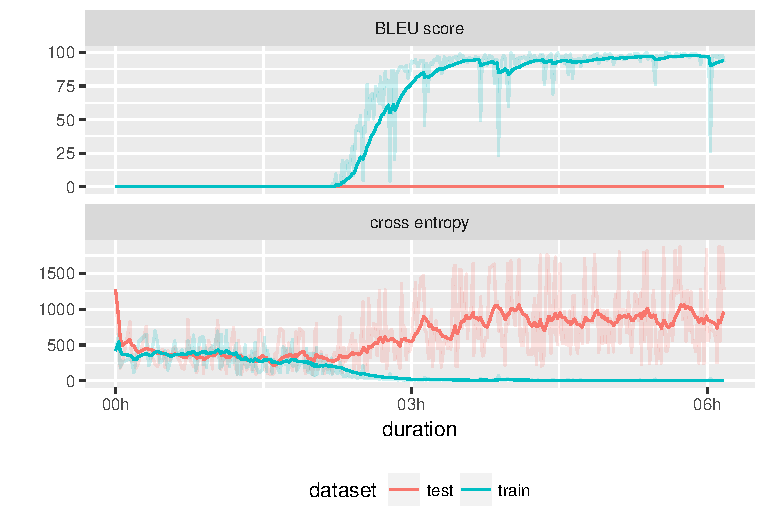
\includegraphics[scale=1]{bytenet/validation-memorize-wmt.pdf}
    \caption{Shows BLEU score and cross entropy loss for the German to English WMT NewsTest dataset. Both training and test measures are calculated on a randomly sampled mini-batch from each dataset.}
\end{figure}

\begin{table}[h]
\centering
\begin{tabular}{r|p{3.3cm} p{3.3cm} p{3.3cm}}
	obs. & source & target & predict\\ \hline
  0  & Zwei Anlagen so nah beieinander: Absicht oder Schildbürgerstreich? & Two sets of lights so close to one another: intentional or just a silly error? & Twi sett of laghand whol sente bly ancther: ind nti sherrons ana is proun, Ral fromere song Broment Rare the bechivathe sounce. \\
  1 & Diese Frage hat Gutachs Bürgermeister gestern klar beantwortet. & Yesterday, Gutacht's Mayor gave a clear answer to this question. & Yeecerdead Gut cht sagay argespoy ane soactwoverung "fverertids the intors in chem fres sact exinberbe s of Mrear).
\end{tabular}
\caption{Source, target and prediction on the training dataset.}
\end{table}

\begin{table}[h]
\centering
\begin{tabular}{r|p{3.3cm} p{3.3cm} p{3.3cm}}
	obs. & source & target & predict\\ \hline
  0  & Zwei Anlagen so nah beieinander: Absicht oder Schildbürgerstreich? & Two sets of lights so close to one another: intentional or just a silly error? & Two sets of Gights so closento ond anotrero forentiog ther Gperbe ties wron the pllis buching thats and and ane. \\
  1 & Diese Frage hat Gutachs Bürgermeister gestern klar beantwortet. & Yesterday, Gutacht's Mayor gave a clear answer to this question. & Yesterday, Guthaltha Meyor gage in ther assuer to the ricesteon deromen to now, aing warr pepe hevern wer a sevembytich.
\end{tabular}
\caption{Source, target and prediction on the test dataset.}
\end{table}

\clearpage
\subsection{WMT Translation Task}

\begin{figure}[H]
    \centering
    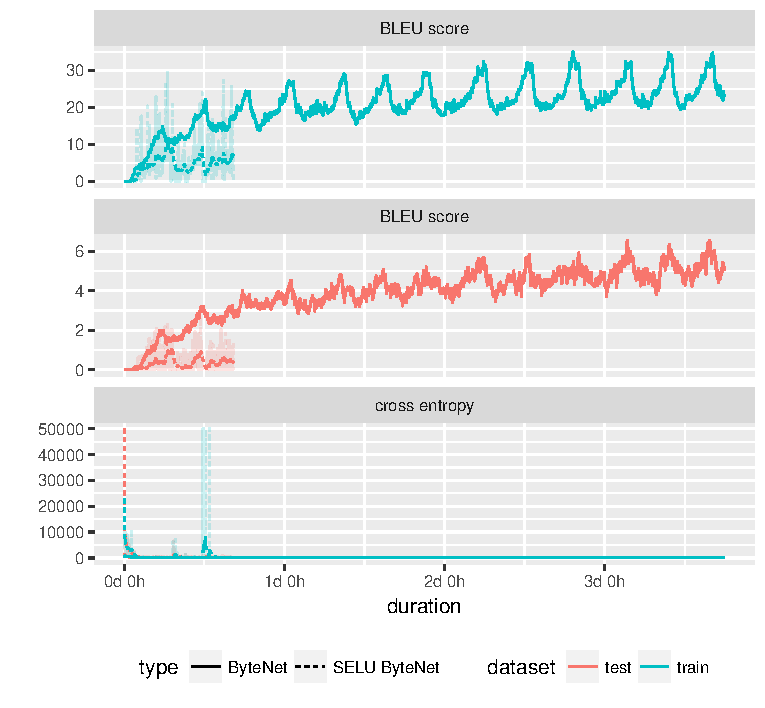
\includegraphics[scale=1]{bytenet/europarl.pdf}
    \caption{Shows misclassification rate on the test dataset and cross entropy loss on the training dataset. The training size is set to 128 observations, likewise for the test dataset. For comparison a the attention model has misclassification rate at 0.51.}
\end{figure}

\subsection{Performance profiling}

\begin{figure}[H]
    \centering
    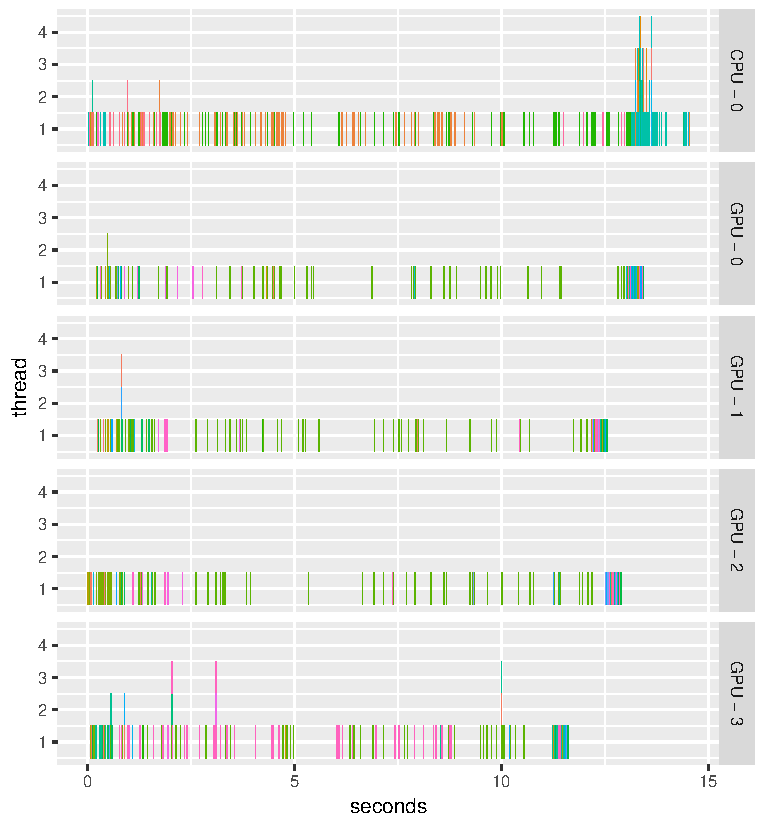
\includegraphics[width=\textwidth]{bytenet/profile-raw.pdf}
    \caption{}
\end{figure}


\begin{figure}[H]
    \centering
    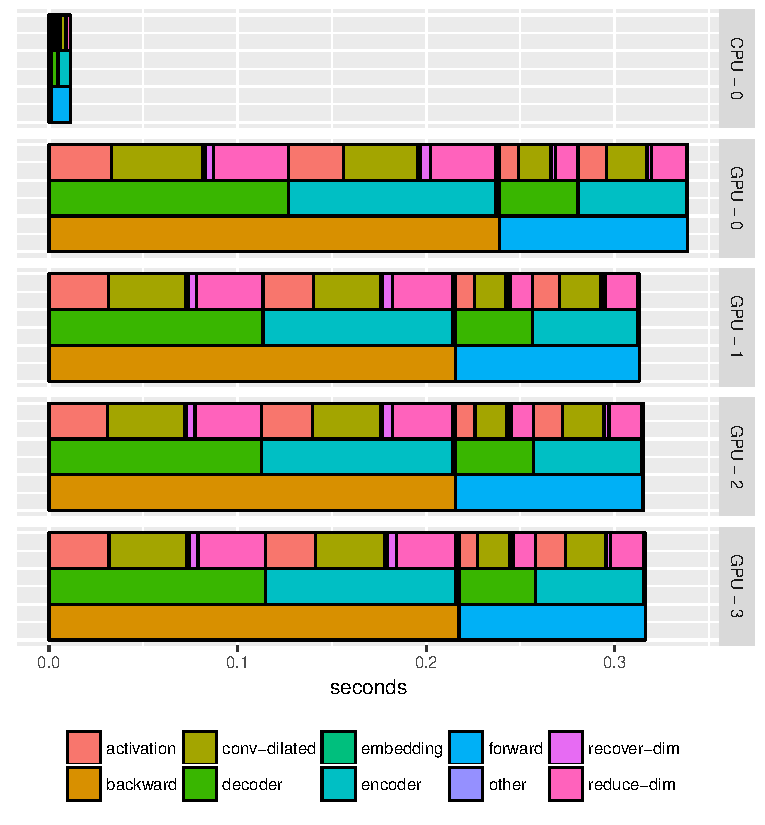
\includegraphics[scale=1]{bytenet/profile-grouped.pdf}
    \caption{}
\end{figure}
